%\section{Defining the neutrino floor/fog by discovery potential}
\section{The neutrino fog}
\label{sec:neutrinofloor}

As direct dark matter searches accumulate ever larger exposures in pursuit of testing smaller interaction cross sections, the expected background from the coherent elastic neutrino-nucleus scattering (CE$\nu$NS) of astrophysical neutrinos increases. For dark matter masses $\gtrsim10$~GeV/$c^2$, the relevant neutrino fluxes are those from $^8$B solar neutrinos, atmospheric neutrinos, and the diffuse supernova background (DSNB) neutrinos. The CE$\nu$NS event rate from each of these is subject to a systematic uncertainty which manifests from the uncertainty on the flux of each neutrino species. In addition, the nuclear recoil energy spectra of these events closely resembles that of the sought after dark matter signal -- this is the case for a spin-independent (SI) dark matter interaction as well as for other couplings/interactions. An example is given in Fig.~\ref{fig:coherent_solarnu_rates}, which shows the SI nuclear recoil rate of a couple of WIMP masses on xenon and argon alongside those of the dominant neutrino backgrounds. 

The effect of these backgrounds -- particularly because of their associated systematic uncertainties and spectral shapes --  will be to reduce the dark matter sensitivity achievable as the experimental exposure grows. This fact lead to the creation of the colloquially known ``neutrino floor": a boundary in the cross section versus dark matter matter mass plane below which a dark matter discovery becomes extremely challenging without further constraints on the neutrino backgrounds. The precise location of this boundary has evolved over the last decade~\cite{Billard:2013qya,Gelmini:2018ogy,OHare:2020lva,OHare:2021utq}, however more recent studies~\cite{OHare:2020lva,OHare:2021utq} have emphasized a crucial point: that astrophysical neutrino backgrounds do not impose a hard limit on physics reach, rather, the effect is more gradual than a single boundary depicts. To reinforce this concept within the community, the term ``neutrino fog" has instead been used to describe the region of dark matter cross sections where neutrino backgrounds begin to inhibit the progress of direct detection searches.

%The effect of these backgrounds -- in particular, because of their associated systematic uncertainties and spectral shapes --  will be to reduce the dark matter sensitivity for each additional increment of experimental exposure that is 
%The effect of these backgrounds -- in particular, because of their associated systematic uncertainties and spectral shapes --  will be to reduce the dark matter sensitivity achievable as the experiment with subsequently increasing exposures.
%The effect of this background will be an increasingly suppressed dark matter cross section reach as the experimental exposure grows: 
%an increasingly suppressed dark matter cross section reach as the experimental exposure grows: 
%\textcolor{red}{now introduce concept of `fog/floor', cite older and newer defintions}
%\textcolor{red}{explain our definition}

\subsection{Defining the neutrino fog}

We choose to adopt the methodology of Ref.~\cite{OHare:2021utq} in defining the neutrino fog region. Specifically, the quantity of interest is the index $n$, defined as the gradient of a hypothetical experiment's median cross section for $3\sigma$ discovery with respect to the exposure:

\begin{equation}
    n = -\bigg( \frac{d \log{\sigma}}{d \log{MT}} \bigg)^{-1}
\end{equation}

%Clearly set out a canonical definition of the neutrino floor/fog/whatever so that we are explicit in this paper, and hopefully becomes the standard definition in the community. Should be independent of technology (other than target isotope) and independent of threshold if possible. 



\begin{figure}
    \centering
    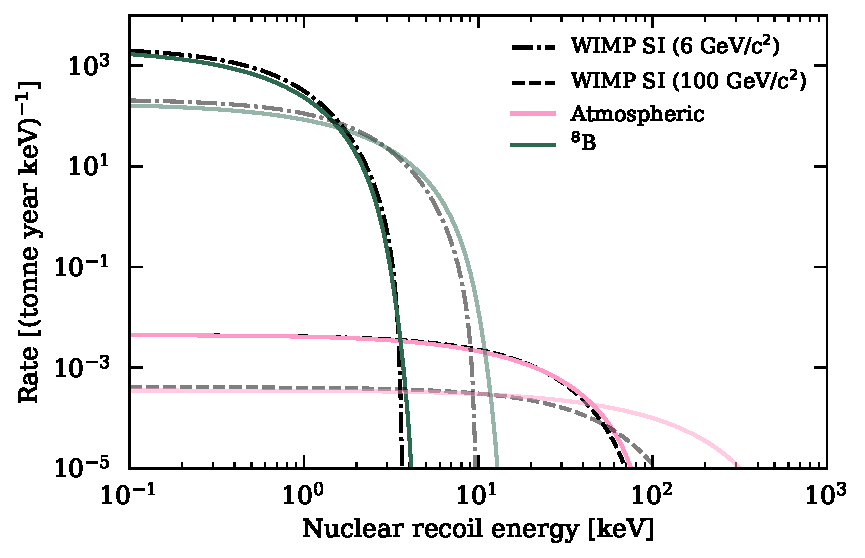
\includegraphics[width=0.75\textwidth]{figures/nu_rates_coherent_combined.pdf}
    \caption{Spectrum of solar-neutrino nuclear recoils scattering on Xe (darker color) and Ar (lighter color). The recoil spectrum for a 6 GeV/$c^2$ (dashed line) and a 100 GeV/$c^2$ (dotted-dashed line) are also given for reference.}
    \label{fig:coherent_solarnu_rates}
\end{figure}


\begin{figure}[tbh]
    \centering
    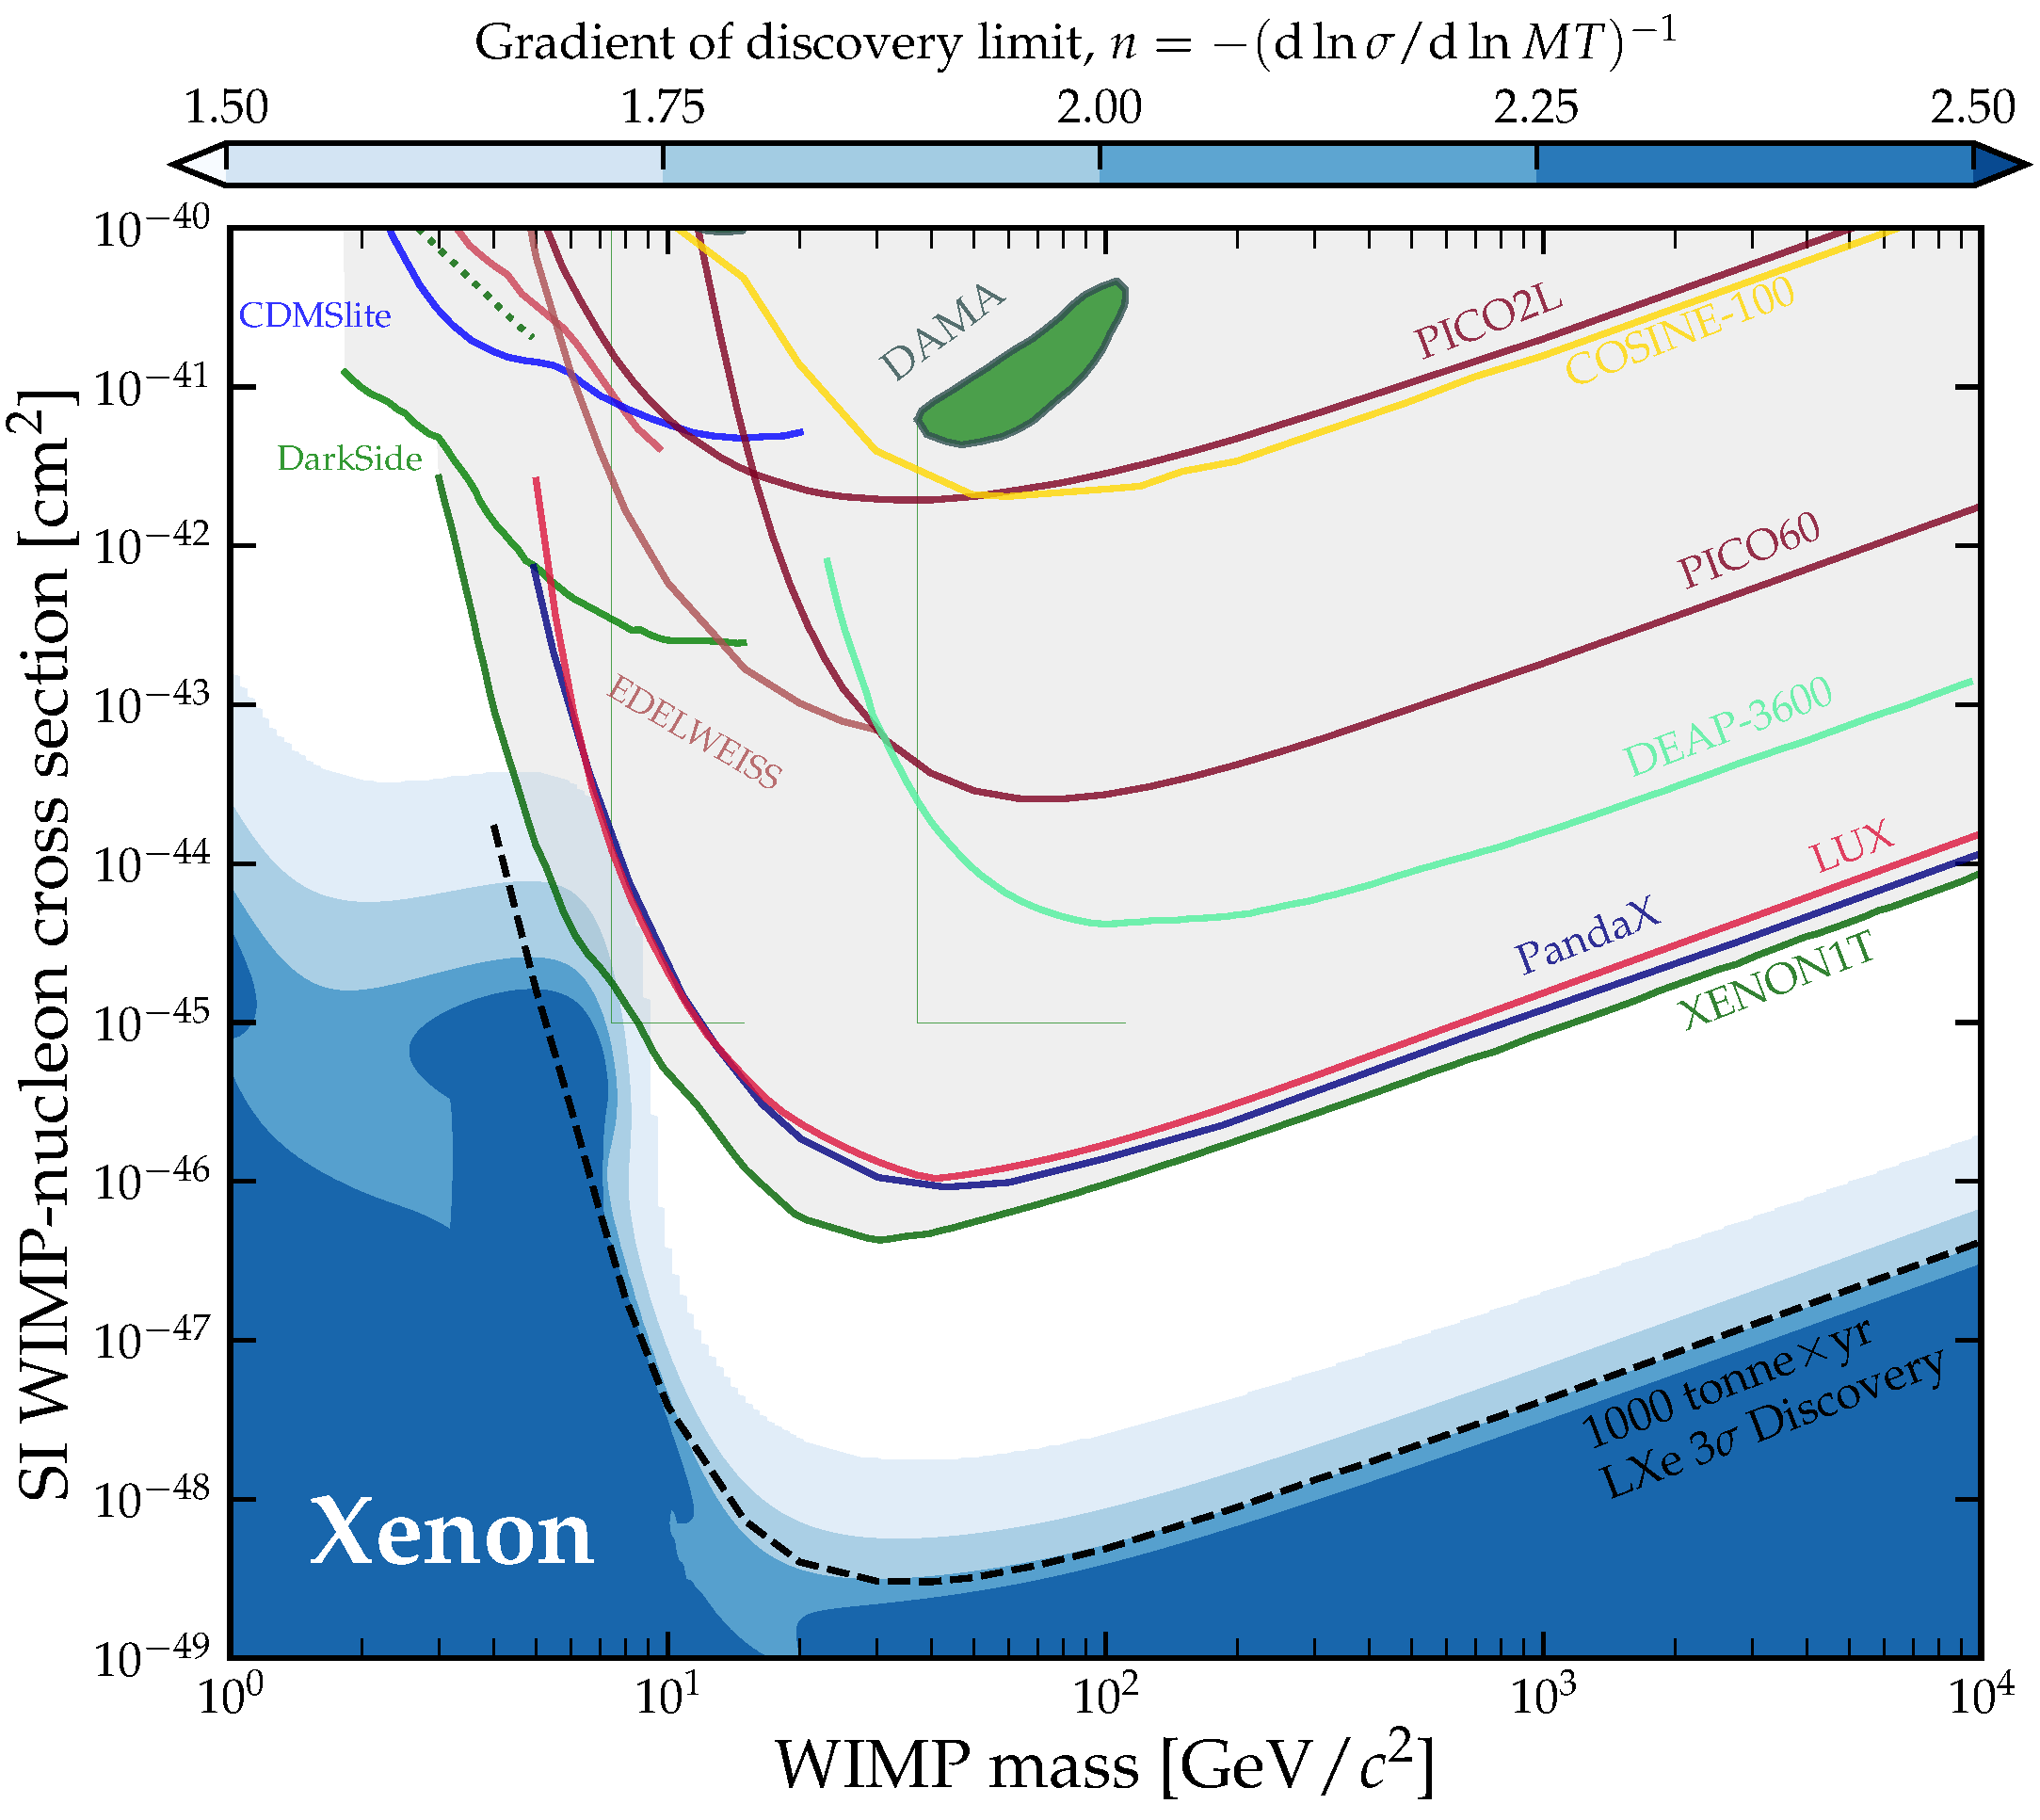
\includegraphics[width=0.75\textwidth]{figures/single_panel_nufog_blues_v3.pdf}
    \caption{\textcolor{red}{subject to change.} Standard spin-independent neutrino floor/fog/whatever for various isotopes.}
    \label{fig:neutrino_floor}
\end{figure}


\subsection{Relating the neutrino floor to EFT couplings}
Lead: David Cerdeno

Highlight EFT couplings that produce signal shapes very different from solar neutrino spectrum, allowing currently-mature-technology detector probe cross sections below the generic spin-dependent neutrino floor. 


